\documentclass{standalone}
\usepackage{tikz}
\usetikzlibrary{
  arrows,
  calc,
  decorations.pathmorphing,
  decorations.pathreplacing,
  decorations.markings,
  fadings,
  positioning,
  shapes,
  arrows.meta
}
\usepgfmodule{oo}

\pgfdeclareradialshading{glow2}{\pgfpoint{0cm}{0cm}}{
  color(0mm)=(white);
  color(2mm)=(white);
  color(8mm)=(black);
  color(10mm)=(black)
}

\begin{tikzfadingfrompicture}[name=glow2 fading]
  \shade [shading=glow2] (0,0) circle (1);
\end{tikzfadingfrompicture}

\definecolor{atomblue}{rgb}{0,0,1}
\definecolor{atomorange}{rgb}{1,0.483,0}

\pgfdeclarelayer{tweezer}
\pgfsetlayers{tweezer,main}
\pgfooclass{tweezer}{
  \method tweezer() {
  }
  \method drawAtom(#1,#2,#3,#4) {
    \fill [#4,path fading=glow2 fading] (#1,#2) circle (#3);
  }
  \method drawNaAtom(#1,#2,#3) {
    \pgfoothis.drawAtom(#1,#2,#3,atomorange);
  }
  \method drawCsAtom(#1,#2,#3) {
    \pgfoothis.drawAtom(#1,#2,#3,blue);
  }
}
\pgfoonew \mytweezer=new tweezer()

\ifpdf
% Ensure reproducible output
\pdfinfoomitdate=1
\pdfsuppressptexinfo=-1
\pdftrailerid{}
\fi

\begin{document}

% Scale figure so that the text in the final plot is consistent with other figures
% note that the figure size needs to be scaled separately.
\begin{tikzpicture}[scale=1.27]
  \node at (0, -4.1) {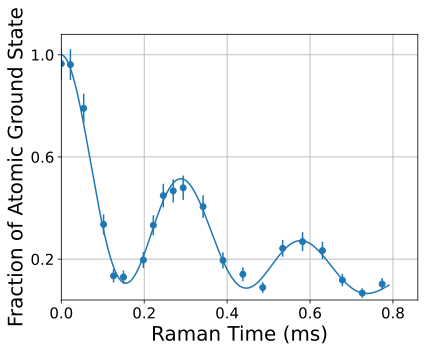
\includegraphics[width=6.75cm]{
      raman_transfer_fit_two_ase_time.pdf}};
  \begin{scope}[shift={(-1.6, -2.6)}]
    \draw plot[samples=200,domain=-0.2:0.2,variable=\x] ({\x + 0.06}, {\x * \x * 10 - 0.17});
    \mytweezer.drawCsAtom(0, 0.06, 0.08)
    \mytweezer.drawNaAtom(0.10, -0.05, 0.065)
  \end{scope}
  \begin{scope}[shift={(-0.45, -3.85)}]
    \draw plot[samples=200,domain=-0.2:0.2,variable=\x] ({\x + 0.06}, {\x * \x * 10 - 0.17});
    \mytweezer.drawCsAtom(0, 0.06, 0.08)
    \mytweezer.drawNaAtom(0.10, -0.05, 0.065)
  \end{scope}
  \begin{scope}[shift={(-1.2, -5.55)}]
    \draw[line width=1] (0, 0) -- (0.15, 0.0);
    \mytweezer.drawCsAtom(0, 0, 0.08)
    \mytweezer.drawNaAtom(0.15, 0, 0.065)
  \end{scope}
\end{tikzpicture}

\end{document}
